\documentclass[aspectratio=169,10pt]{beamer}

\usetheme{Madrid}
\usecolortheme{default}
\setbeamertemplate{navigation symbols}{}

\usepackage{graphicx}
\usepackage{booktabs}
\usepackage{tabularx}
\usepackage{array}
\usepackage{ragged2e}
\usepackage{amsmath}
\usepackage{xcolor}
\usepackage{hyperref}

\graphicspath{{figures/}}

\definecolor{BerkeleyBlue}{RGB}{0,50,98}
\definecolor{BerkeleyLightBlue}{RGB}{59,126,161}
\definecolor{CaliforniaGold}{RGB}{253,181,21}
\definecolor{BugRed}{RGB}{183,38,46}
\definecolor{Fog}{RGB}{232,238,244}
\definecolor{Slate}{RGB}{91,111,130}
\definecolor{ForestGreen}{RGB}{42,127,98}
\definecolor{BodyText}{RGB}{27,39,51}

\setbeamercolor{palette primary}{bg=BerkeleyBlue,fg=white}
\setbeamercolor{palette secondary}{bg=BerkeleyLightBlue,fg=white}
\setbeamercolor{palette tertiary}{bg=CaliforniaGold,fg=BerkeleyBlue}
\setbeamercolor{frametitle}{fg=BerkeleyBlue,bg=white}
\setbeamercolor{title}{fg=BerkeleyBlue}
\setbeamercolor{structure}{fg=BerkeleyBlue}
\setbeamercolor{block title}{bg=BerkeleyBlue,fg=white}
\setbeamercolor{block body}{bg=Fog,fg=BodyText}
\setbeamercolor{alerted text}{fg=BugRed}
\hypersetup{colorlinks=true,urlcolor=BerkeleyLightBlue,linkcolor=BerkeleyBlue}

% Auto-generated by docs/generate_drone_race_progress_assets.py
\newcommand{\EvidenceRunID}{\texttt{dwn4jigo}}
\newcommand{\EvidenceRunURL}{https://wandb.ai/ee106b/omnidrones/runs/dwn4jigo}
\newcommand{\LapCompletionPct}{73.6\%}
\newcommand{\GatesPerEpisode}{9.86}
\newcommand{\LapTimeSeconds}{13.18\,s}
\newcommand{\MeanSpeedMs}{4.77\,m/s}
\newcommand{\MaxSpeedMs}{10.11\,m/s}
\newcommand{\CrashRatePct}{22.9\%}
\newcommand{\EntropyCoef}{0.00197}
\newcommand{\CurriculumPhase}{2}
\newcommand{\AccuracyEMA}{0.733}
\newcommand{\GateElevenCrosses}{1.505}
\newcommand{\PhaseOneFramesM}{29.9M}
\newcommand{\PhaseTwoFramesM}{195.6M}


\newcommand{\metricbox}[2]{%
  \begin{beamercolorbox}[wd=\linewidth,sep=0.5ex,rounded=true,shadow=false]{block body}
    {\large\bfseries #1}\\[-0.1em]
    {\small #2}
  \end{beamercolorbox}
}

\title{\textbf{UC Berkeley EECS DroneRace Progress}}
\subtitle{Code-backed RL training analysis grounded in the current repo and W\&B evidence run \EvidenceRunID}
\author{EECS106B DroneRace Project}
\date{\today}

\begin{document}

\begin{frame}
  \titlepage
  \vspace{-1.1em}
  \begin{beamercolorbox}[wd=\linewidth,sep=0.6ex,rounded=true]{block body}
    \small
    We train an Iris quadrotor to complete a 13-gate race track in Isaac Sim using a PPO pipeline that is deliberately accuracy-first before it becomes speed-focused.
    \hfill\href{\EvidenceRunURL}{\texttt{wandb.ai/.../dwn4jigo}}
  \end{beamercolorbox}
\end{frame}

\begin{frame}{Task and Track}
  \begin{columns}[T,totalwidth=\textwidth]
    \begin{column}{0.64\textwidth}
      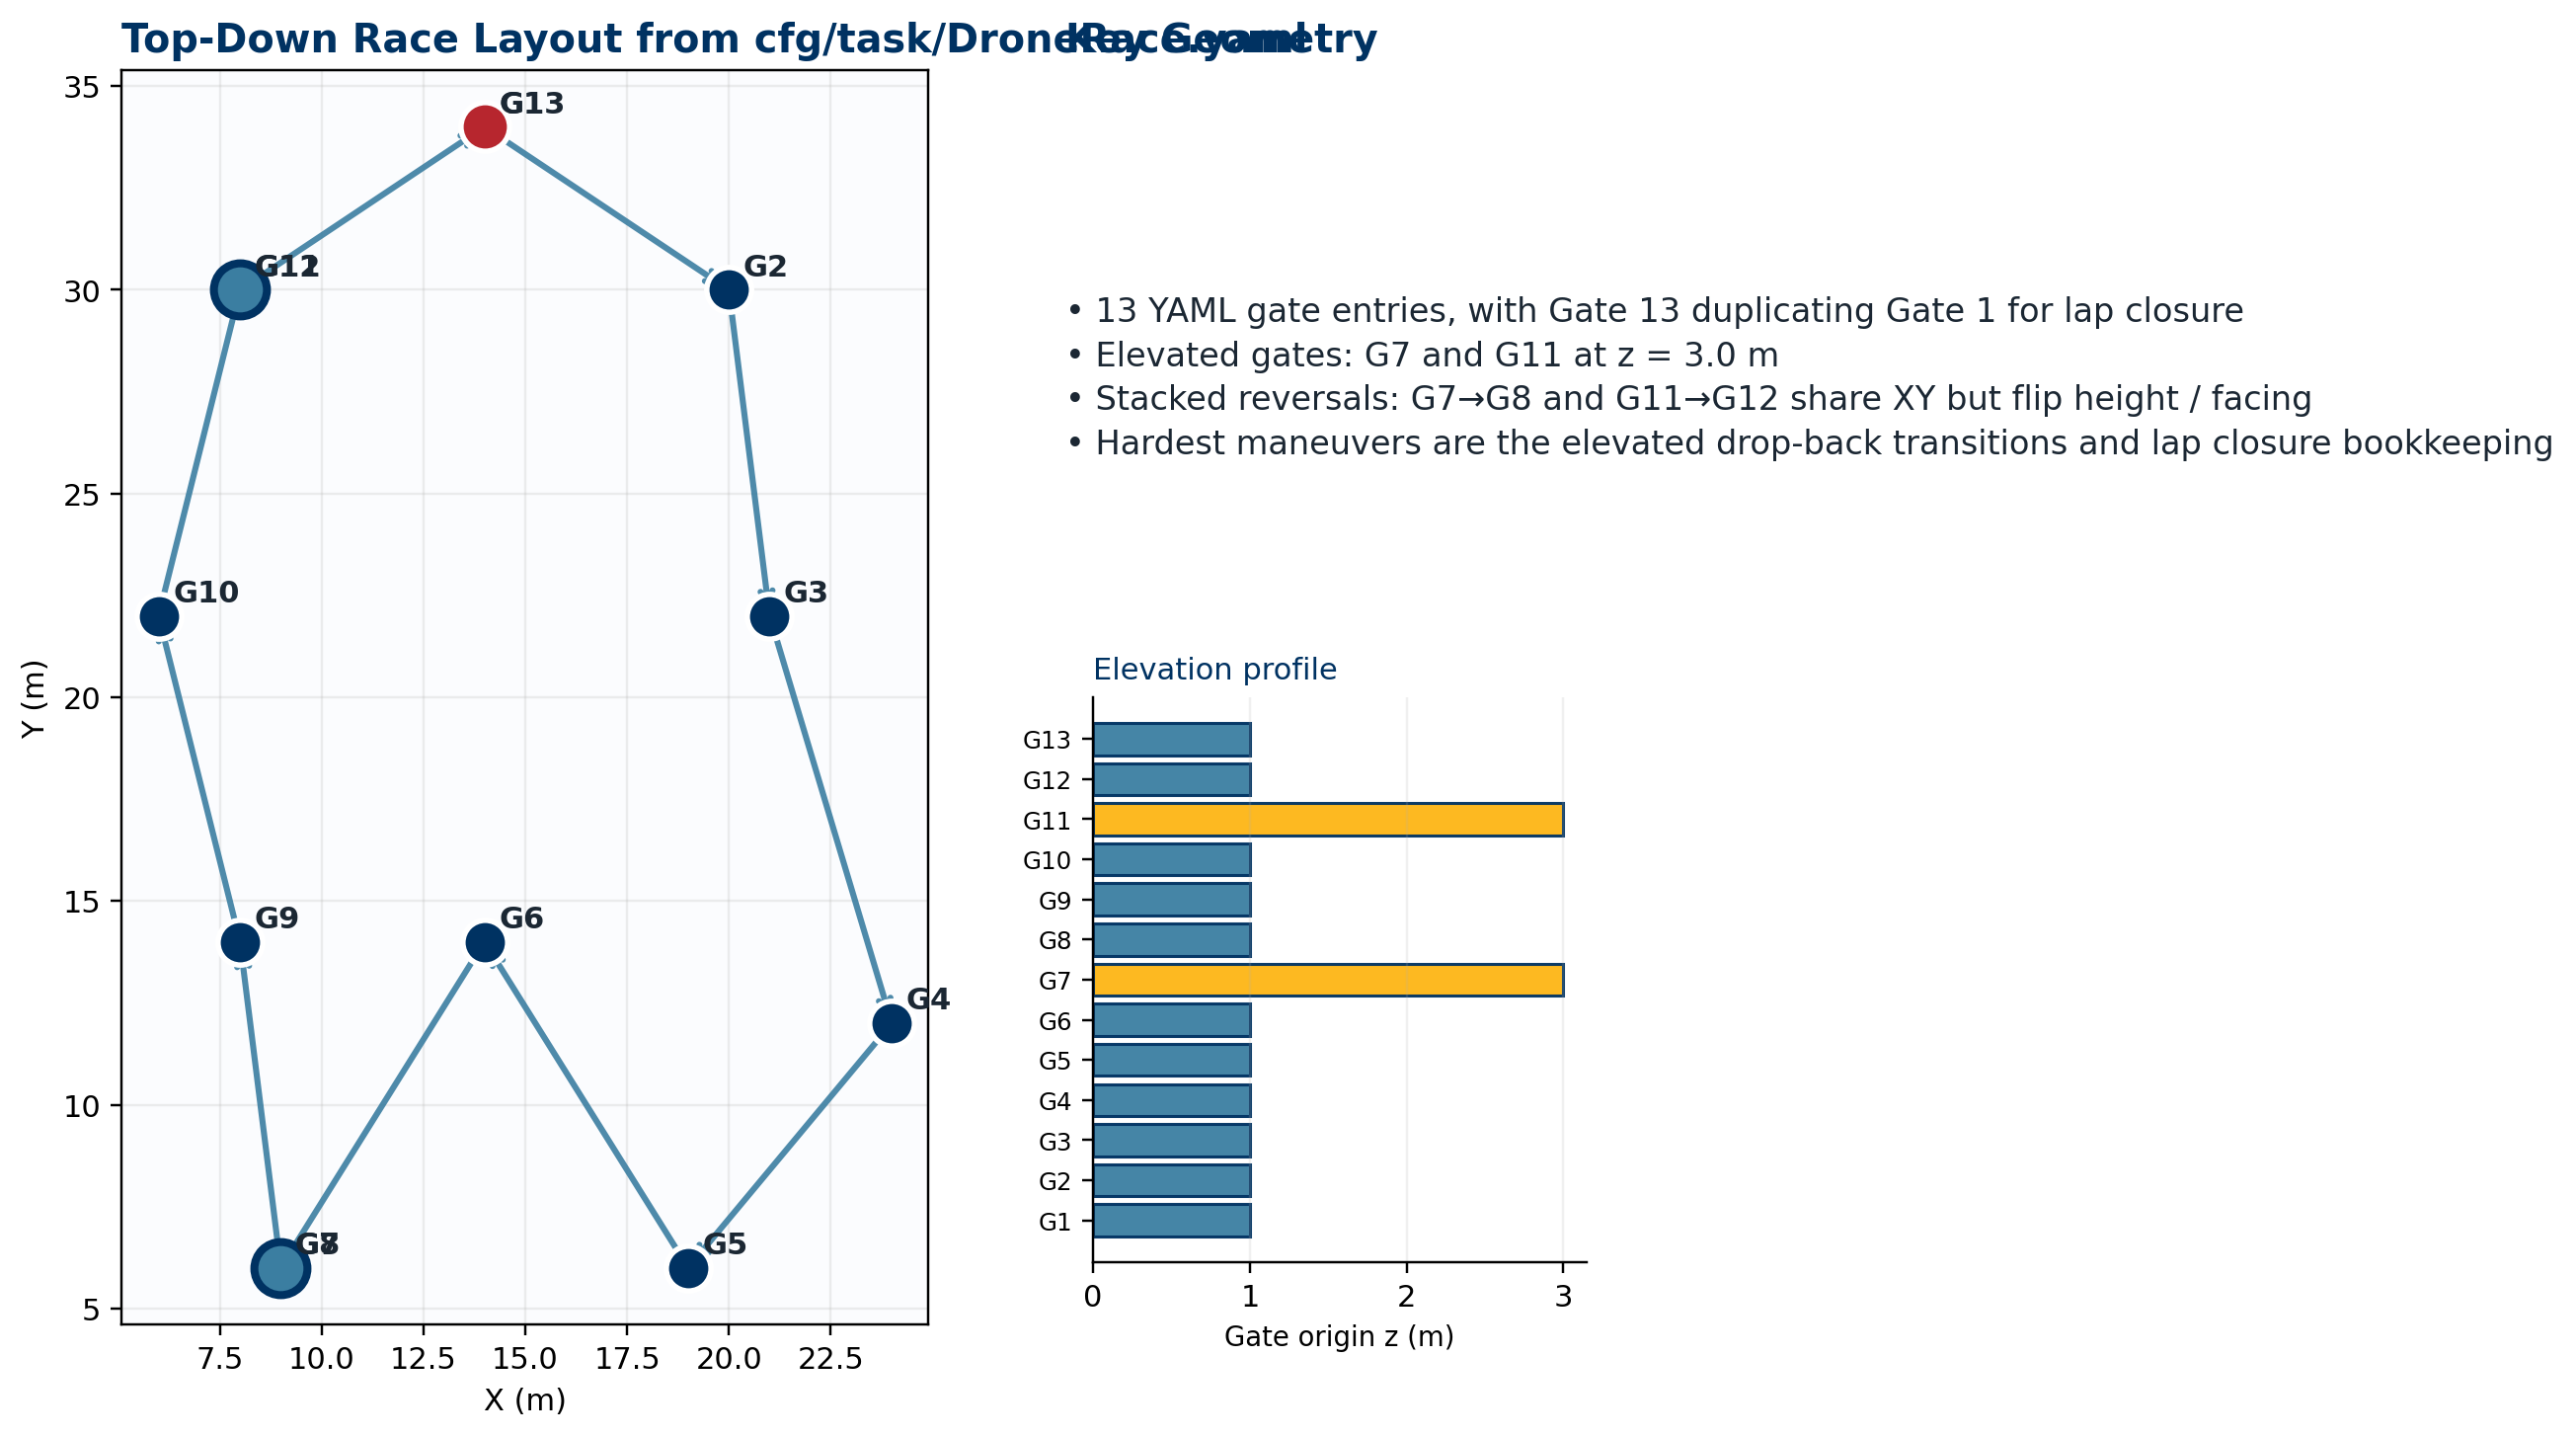
\includegraphics[width=\linewidth]{drone_race_progress_track_schematic.png}
    \end{column}
    \begin{column}{0.34\textwidth}
      \begin{block}{What makes this course hard}
        \scriptsize
        \begin{itemize}
          \item 13 YAML gate entries, with Gate 13 duplicating Gate 1 only for lap closure.
          \item Elevated gates 7 and 11 force climb-drop maneuvers instead of flat turns.
          \item Gates 7$\rightarrow$8 and 11$\rightarrow$12 share XY coordinates, so the policy must reverse locally.
        \end{itemize}
      \end{block}
      \vspace{-0.35em}
      \begin{alertblock}{Interpretation}
        \scriptsize
        This is a sequence-legal race, not just waypoint chasing: crossing the wrong gate, or the right gate from the wrong local geometry, should not count.
      \end{alertblock}
    \end{column}
  \end{columns}
\end{frame}

\begin{frame}{Training System Overview}
  \begin{columns}[T,totalwidth=\textwidth]
    \begin{column}{0.60\textwidth}
      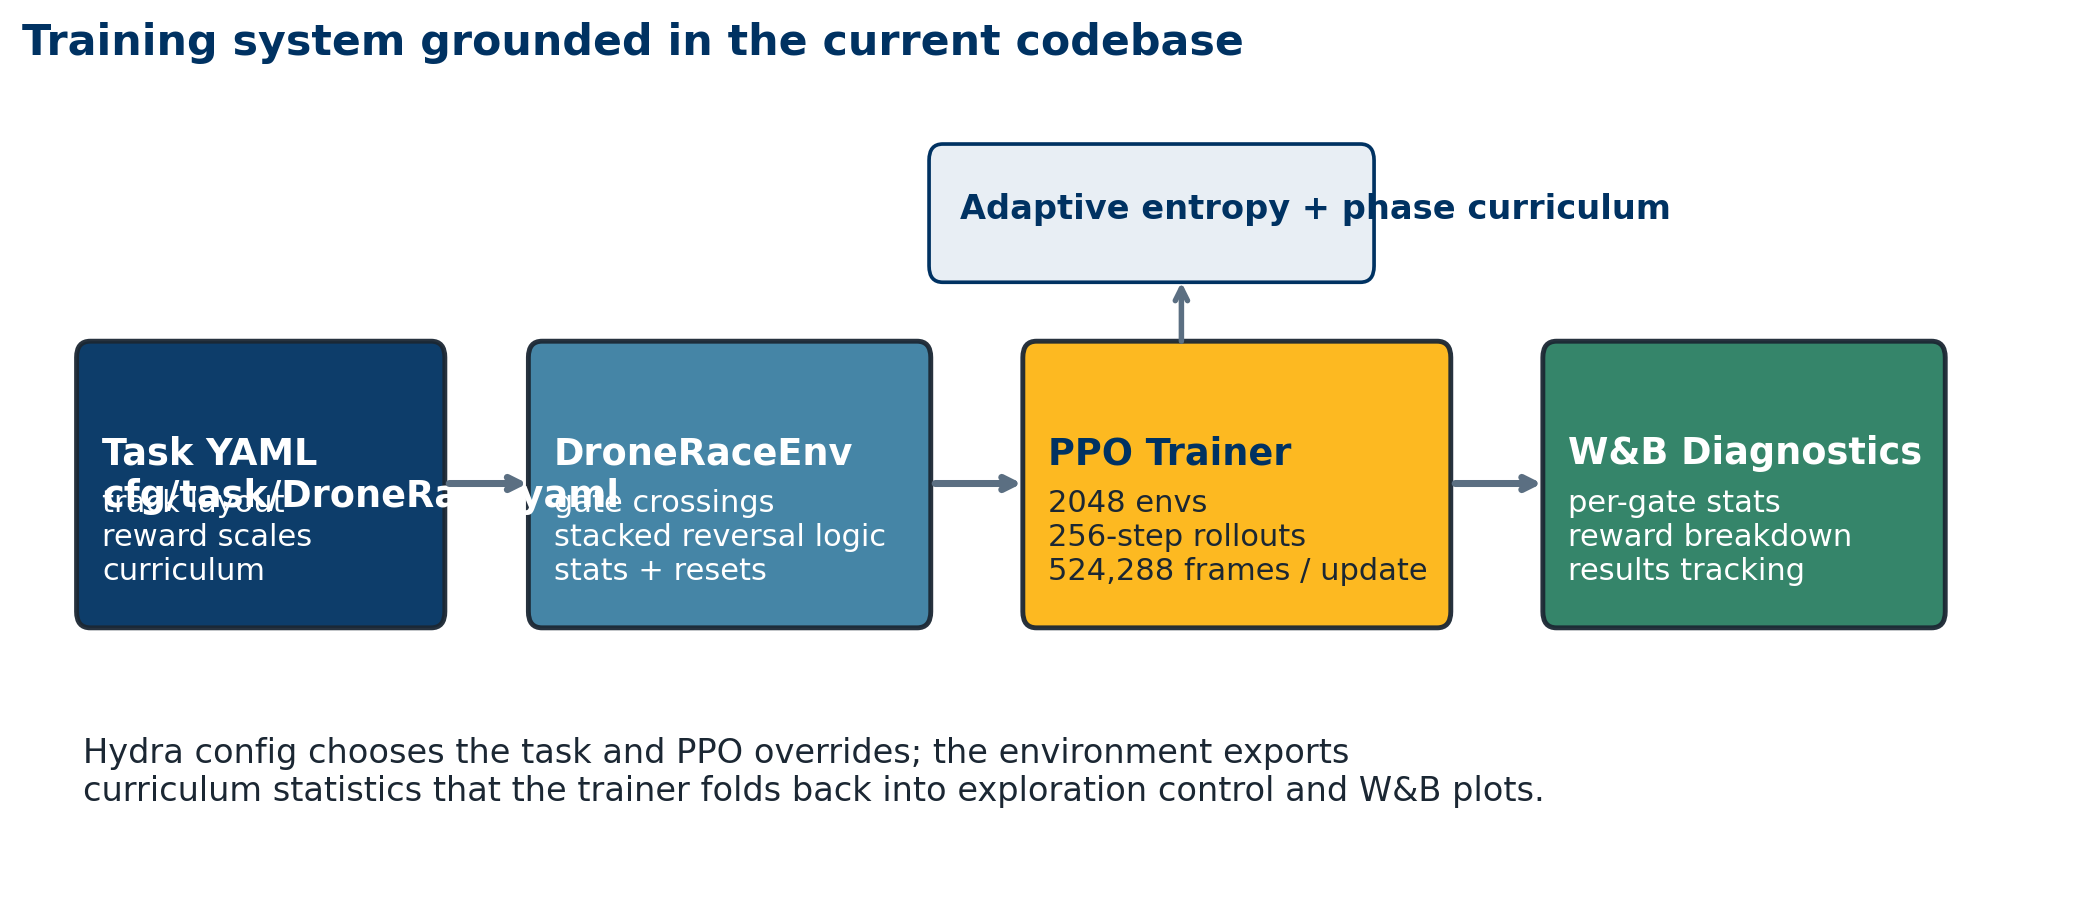
\includegraphics[width=\linewidth]{drone_race_progress_pipeline.png}
    \end{column}
    \begin{column}{0.38\textwidth}
      \begin{block}{Pipeline facts}
        \small
        \begin{itemize}
          \item \texttt{task=DroneRace} loads the task YAML, which then merges \texttt{ppo\_cfg: DroneRace.yaml}.
          \item The active evidence run uses 2048 environments and 256-step rollouts.
          \item Each PPO update therefore consumes 524{,}288 environment frames.
          \item The environment exports curriculum, reset, and per-gate statistics directly into W\&B.
        \end{itemize}
      \end{block}
    \end{column}
  \end{columns}
\end{frame}

\begin{frame}{Adaptive Entropy Algorithm}
  \begin{columns}[T,totalwidth=\textwidth]
    \begin{column}{0.62\textwidth}
      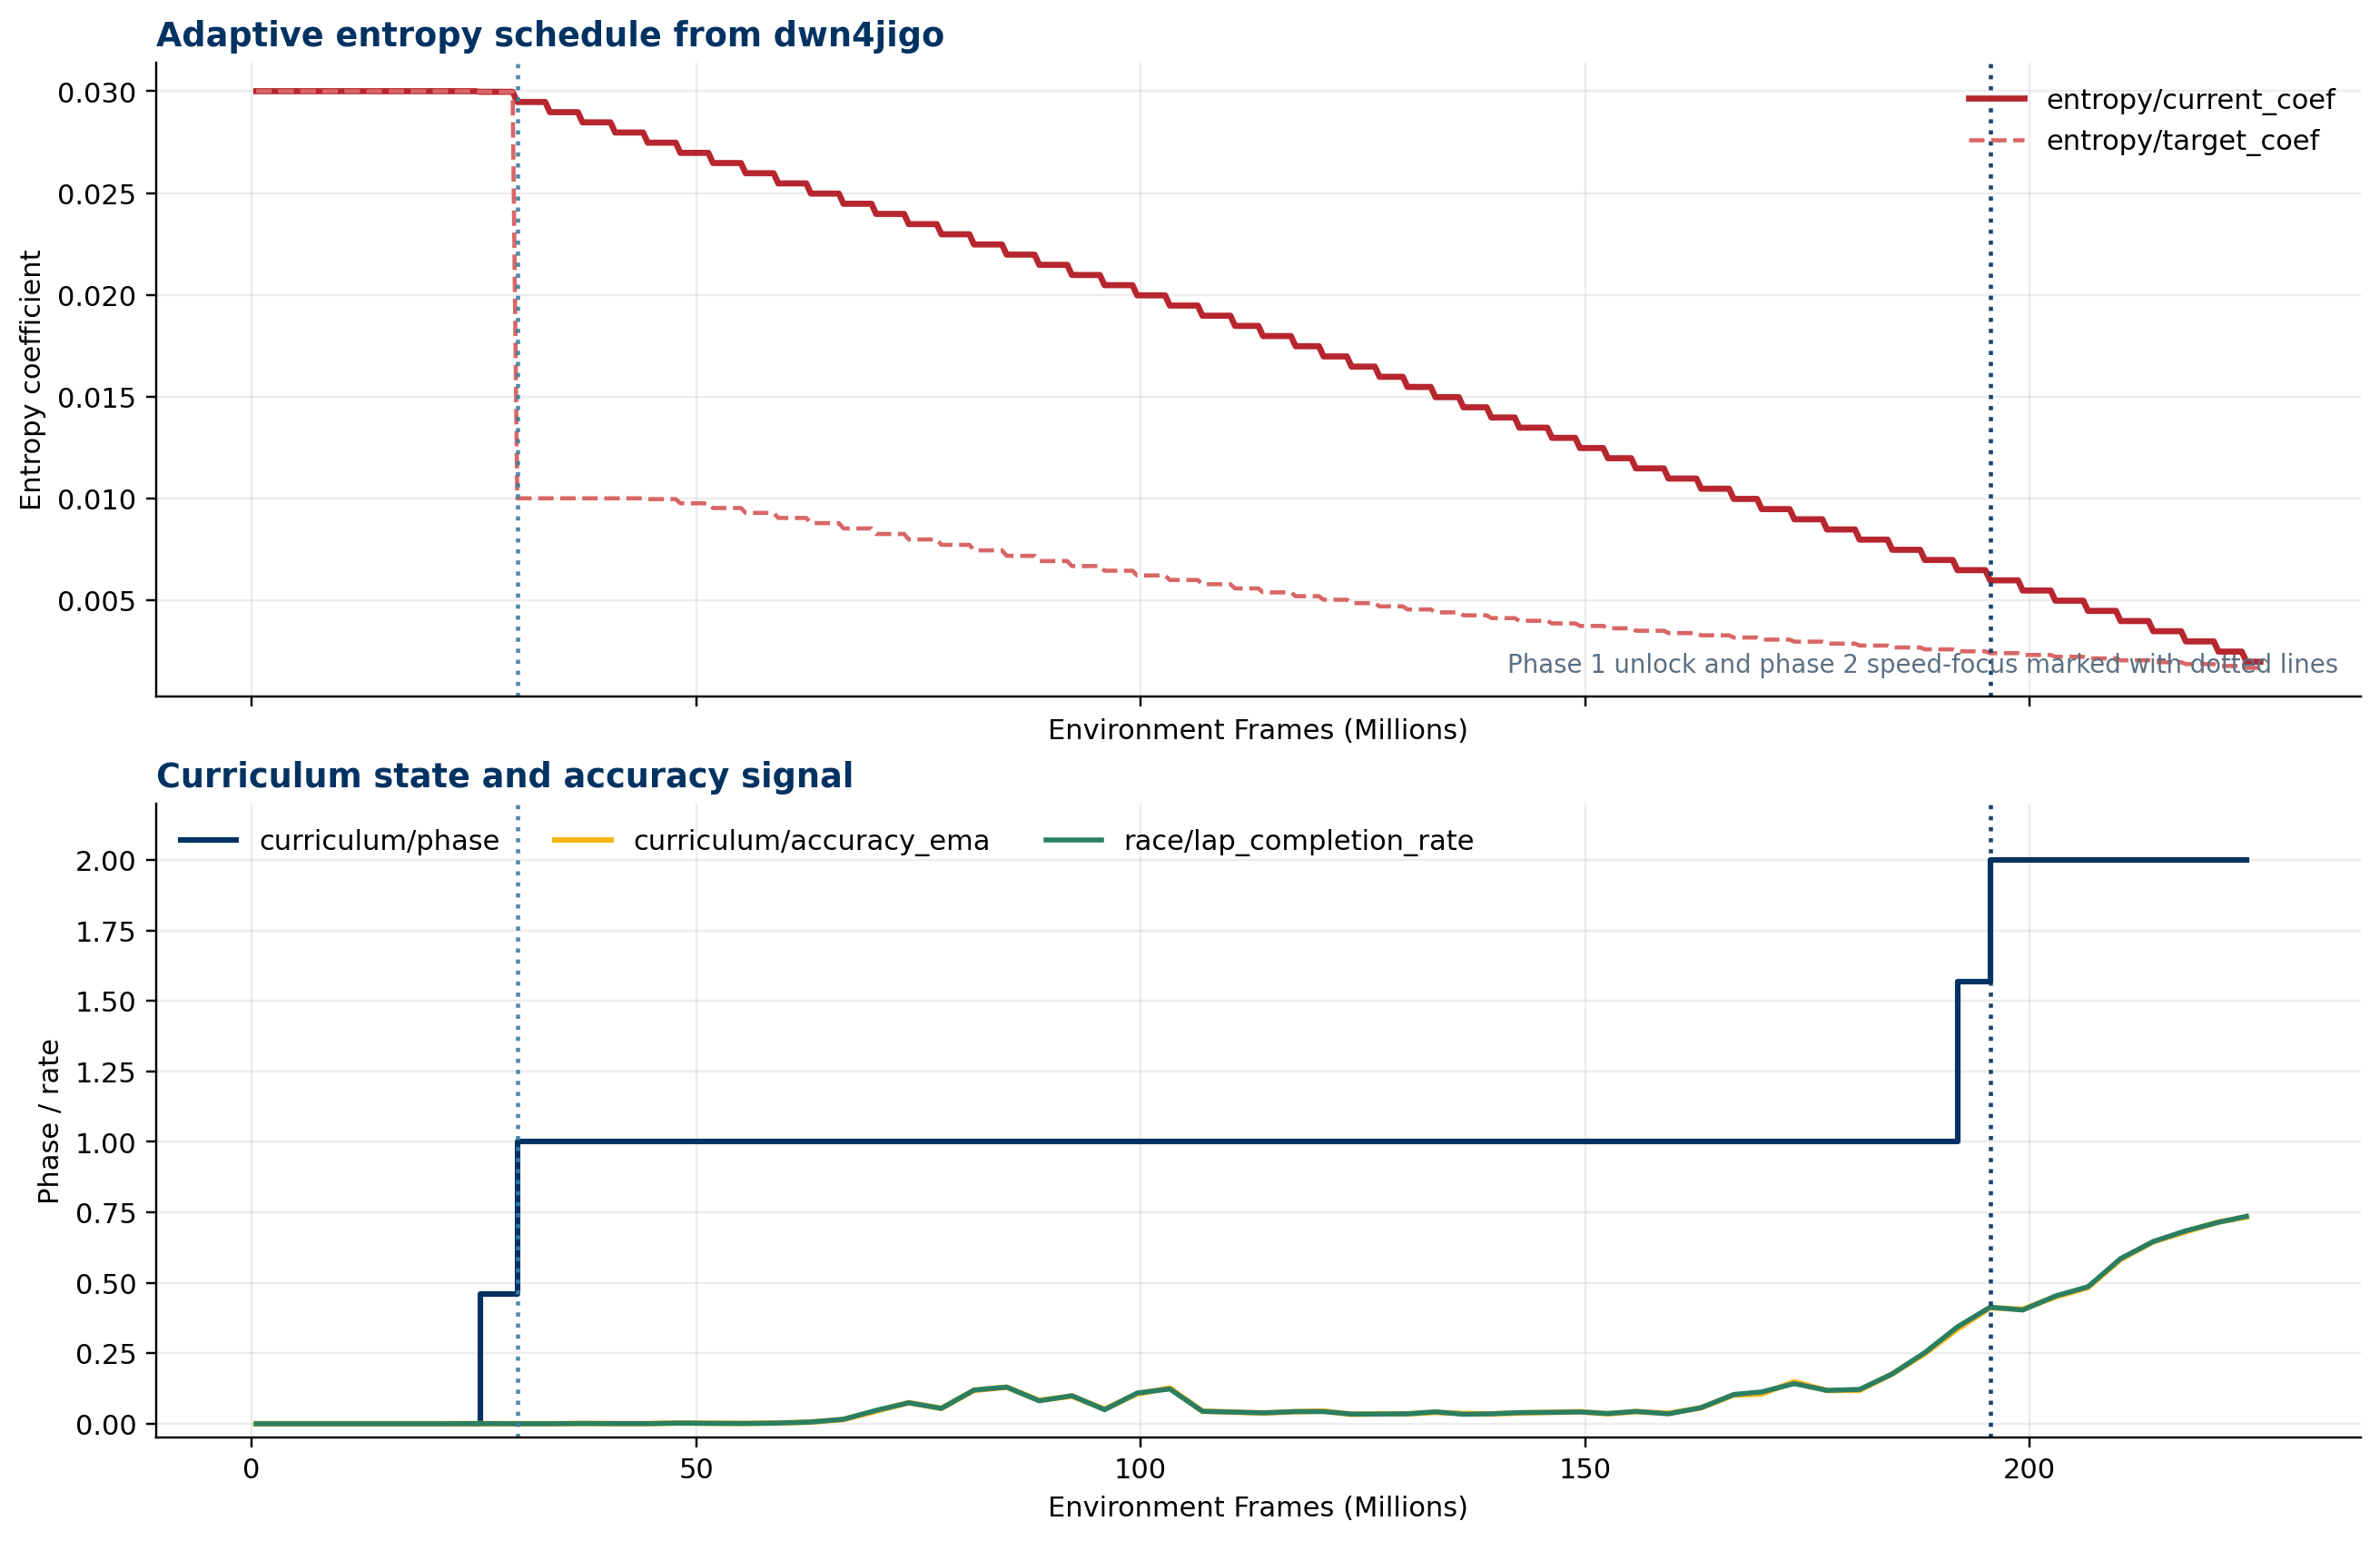
\includegraphics[width=\linewidth]{drone_race_progress_entropy_curriculum.png}
    \end{column}
    \begin{column}{0.36\textwidth}
      \begin{block}{Schedule in code}
        \small
        \[
        \resizebox{0.98\linewidth}{!}{$\alpha_{\text{target}}=\alpha_{\max}-\frac{\text{accuracy EMA}}{\text{unlock rate}}\left(\alpha_{\max}-\alpha_{\min}\right)$}
        \]
        Phase 0 keeps exploration high, phase 1 rebumps entropy when the objective shifts toward speed, and phase 2 decays toward a calmer policy.
      \end{block}
      \begin{block}{Exact run settings}
        \scriptsize
        \begin{itemize}
          \item \texttt{phase0\_coef\_max = 0.03}
          \item \texttt{phase0\_coef\_min = 0.002}
          \item \texttt{phase1\_rebump\_coef = 0.01}
          \item \texttt{phase1\_coef\_min = 0.0005}
          \item Current run ended at \texttt{\EntropyCoef}
        \end{itemize}
      \end{block}
    \end{column}
  \end{columns}
\end{frame}

\begin{frame}{Other Algorithmic Choices Beyond Vanilla PPO}
  \begin{columns}[T,totalwidth=\textwidth]
    \begin{column}{0.54\textwidth}
      \begin{block}{Why this is not default PPO}
        \small
        \begin{itemize}
          \item Long-horizon credit assignment with \texttt{gamma = 0.998} and \texttt{gae\_lambda = 0.95}.
          \item Privileged actor and critic inputs are enabled, so the policy can exploit simulation-only intrinsics during training.
          \item The critic uses Huber loss, layer normalization, and a wider architecture to stabilize sparse ordered-lap rewards.
          \item We keep the rollout long enough to cover multiple gate interactions per batch instead of learning from tiny fragments.
        \end{itemize}
      \end{block}
    \end{column}
    \begin{column}{0.44\textwidth}
      \begin{block}{Compact objective reminder}
        \small
        \[
        \resizebox{0.98\linewidth}{!}{$L^{\text{CLIP}}(\theta)=\mathbb{E}\left[\min\!\left(r_t(\theta)\hat A_t,\operatorname{clip}(r_t(\theta),1-\epsilon,1+\epsilon)\hat A_t\right)\right]$}
        \]
        \vspace{-0.7em}
        \begin{itemize}
          \item \texttt{clip\_param = 0.2}
          \item \texttt{ppo\_epochs = 10}
          \item \texttt{num\_minibatches = 16}
        \end{itemize}
      \end{block}
      \begin{alertblock}{Practical takeaway}
        \small
        The goal was to make PPO act like a serious racing trainer, not a homework default.
      \end{alertblock}
    \end{column}
  \end{columns}
\end{frame}

\begin{frame}{Reward Design}
  \begin{columns}[T,totalwidth=\textwidth]
    \begin{column}{0.54\textwidth}
      \scriptsize
      \setlength{\tabcolsep}{3pt}
      \begin{tabular}{>{\RaggedRight\arraybackslash}p{0.33\linewidth}>{\RaggedRight\arraybackslash}p{0.17\linewidth}>{\RaggedRight\arraybackslash}p{0.34\linewidth}}
        \toprule
        \textbf{Term} & \textbf{Value} & \textbf{Role} \\
        \midrule
        Gate passage & 60 & Sparse legal crossing reward \\
        Gate sequence & 20$\times$ streak & Ordered chain bonus \\
        Lap completion & 500 & Full-course objective \\
        Lap speed bonus & 300 & Time-aware phase-1/2 bonus \\
        Progress shaping & 1.0 & Small racing-line guidance \\
        Speed shaping & 0.25 / 0.75 & Delayed dense speed pressure \\
        Altitude penalty & 0.5 & Elevated-gate height matching \\
        Centering penalty & 0.03 & Discourage fly-bys near the plane \\
        Crash penalty & 80 & Punish divergence or collision \\
        \bottomrule
      \end{tabular}
      \vspace{0.15em}
      \begin{alertblock}{Design principle}
        \scriptsize
        Ordered gate legality must dominate dense shaping, otherwise the policy can learn to fly fast in roughly the right direction without actually racing the course.
      \end{alertblock}
    \end{column}
    \begin{column}{0.44\textwidth}
      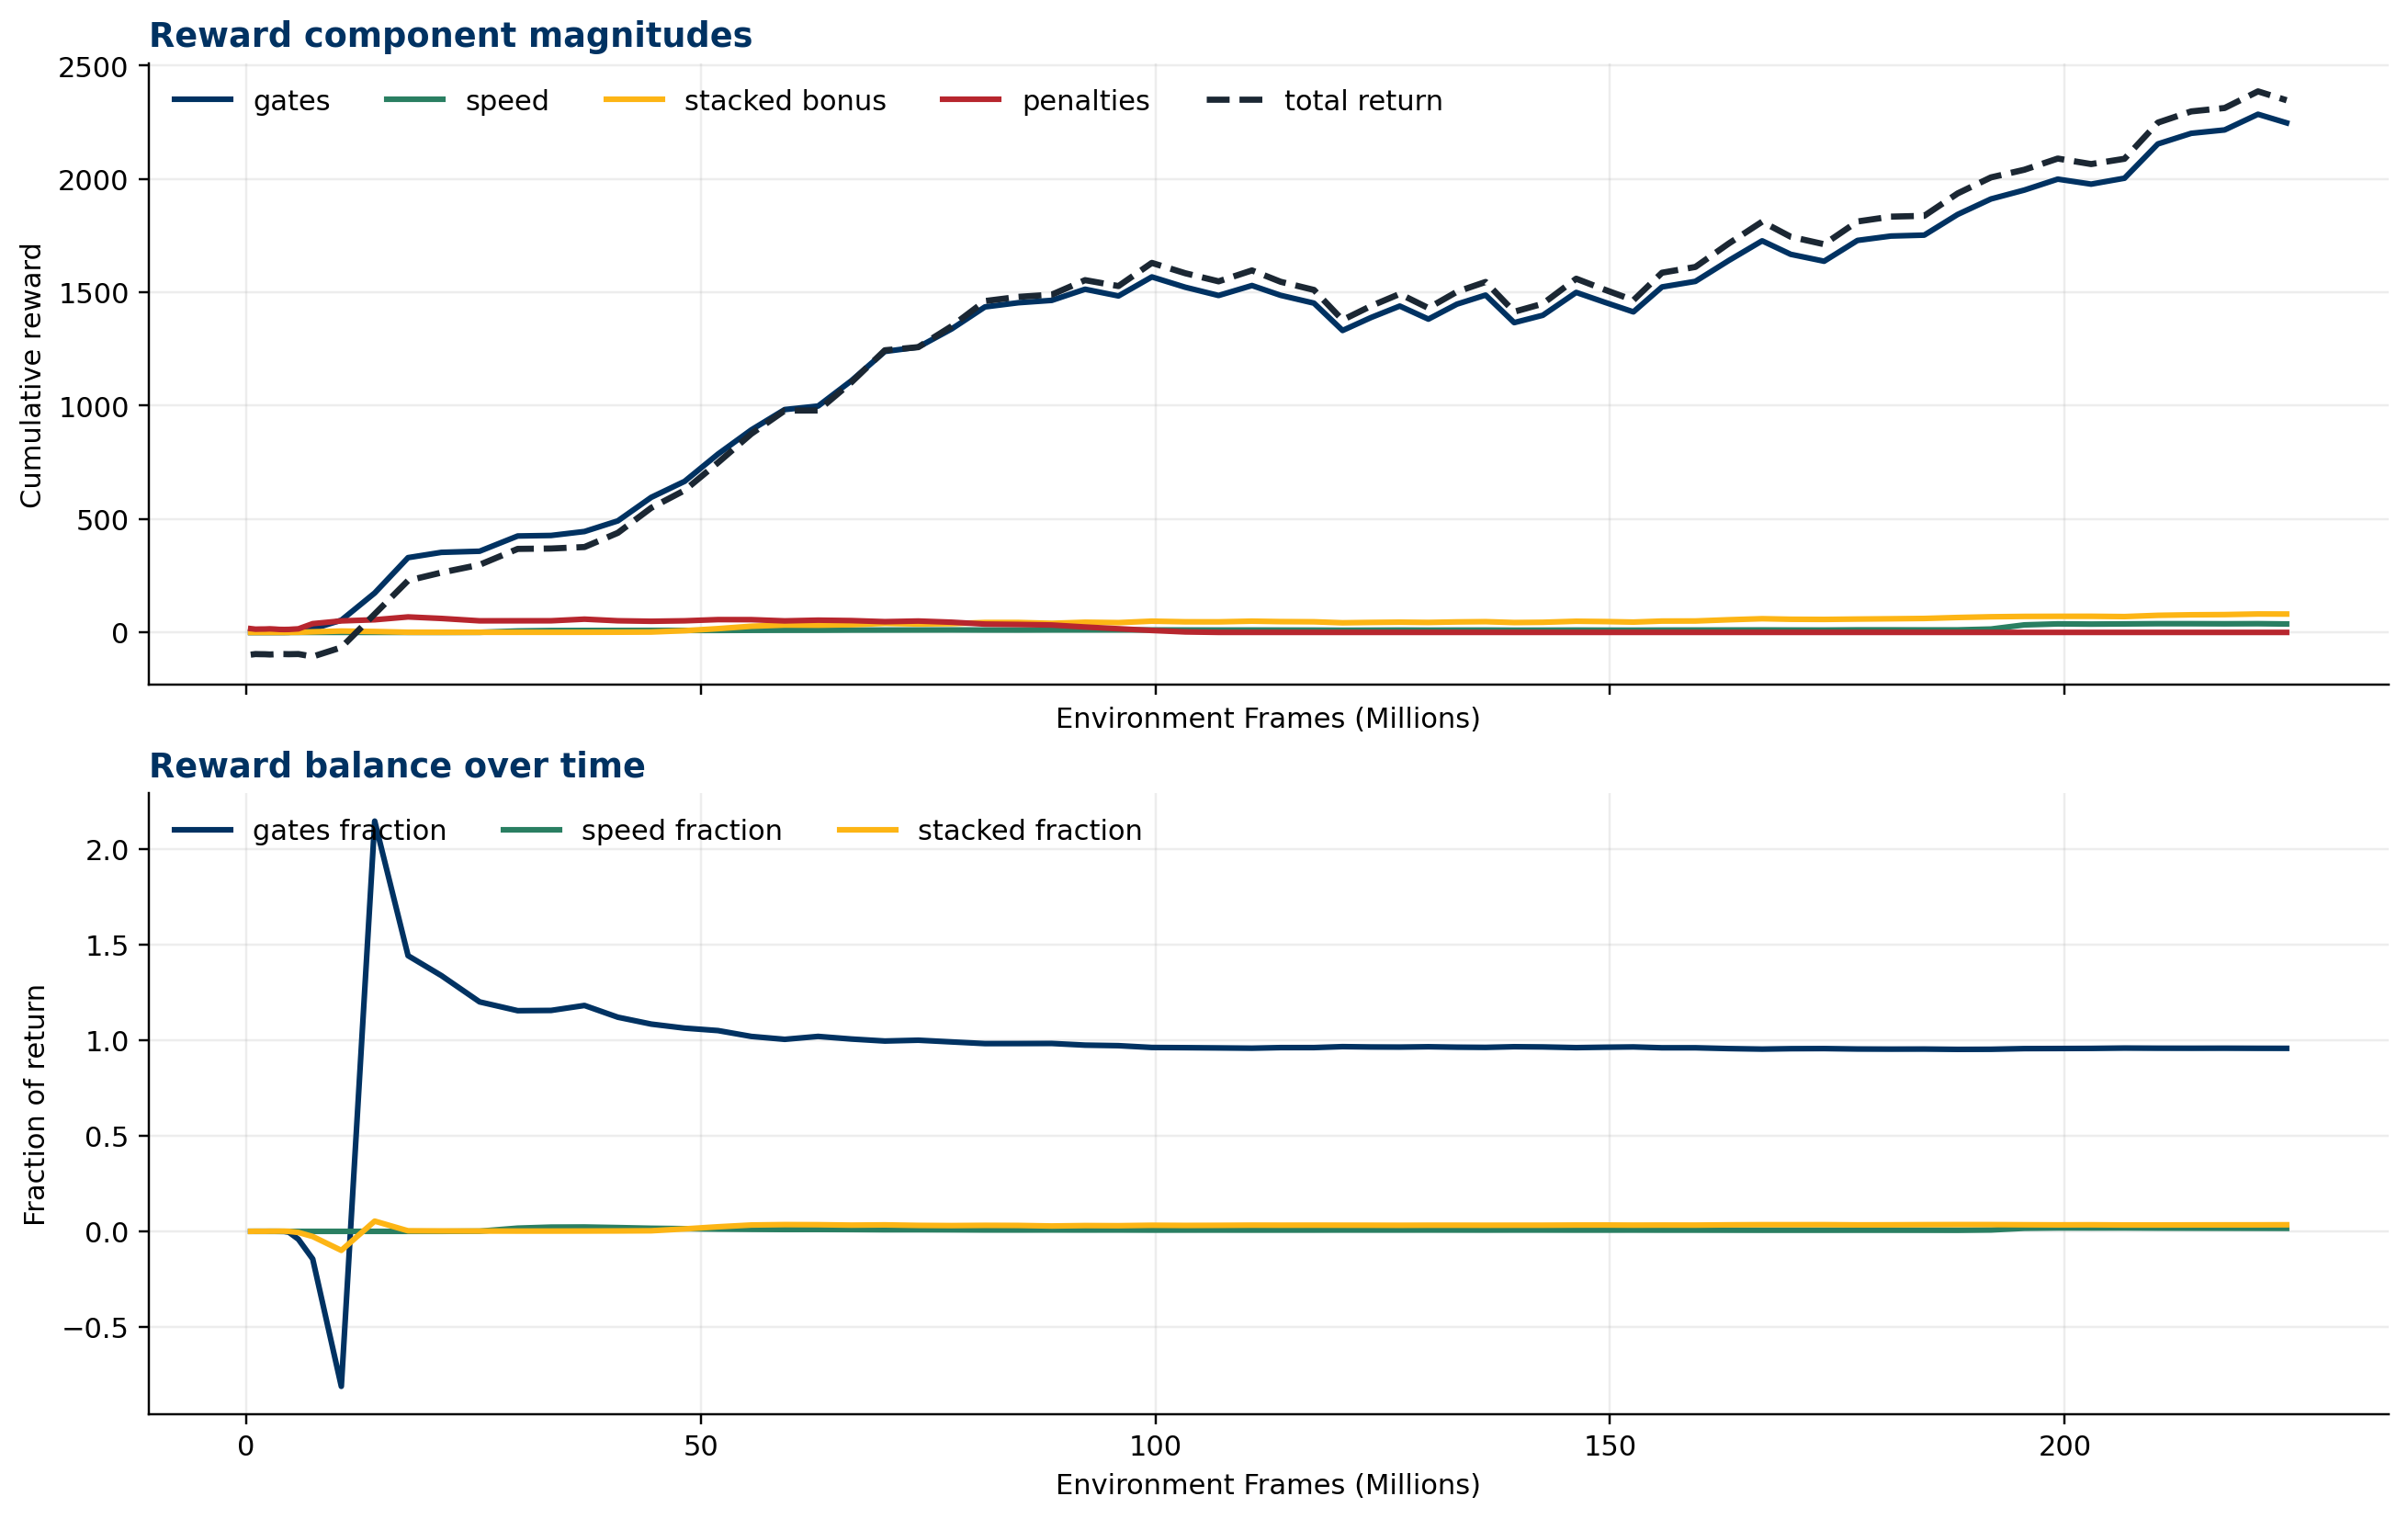
\includegraphics[width=\linewidth]{drone_race_progress_reward_components.png}
    \end{column}
  \end{columns}
\end{frame}

\begin{frame}{Curriculum and Reset Distribution}
  \begin{columns}[T,totalwidth=\textwidth]
    \begin{column}{0.58\textwidth}
      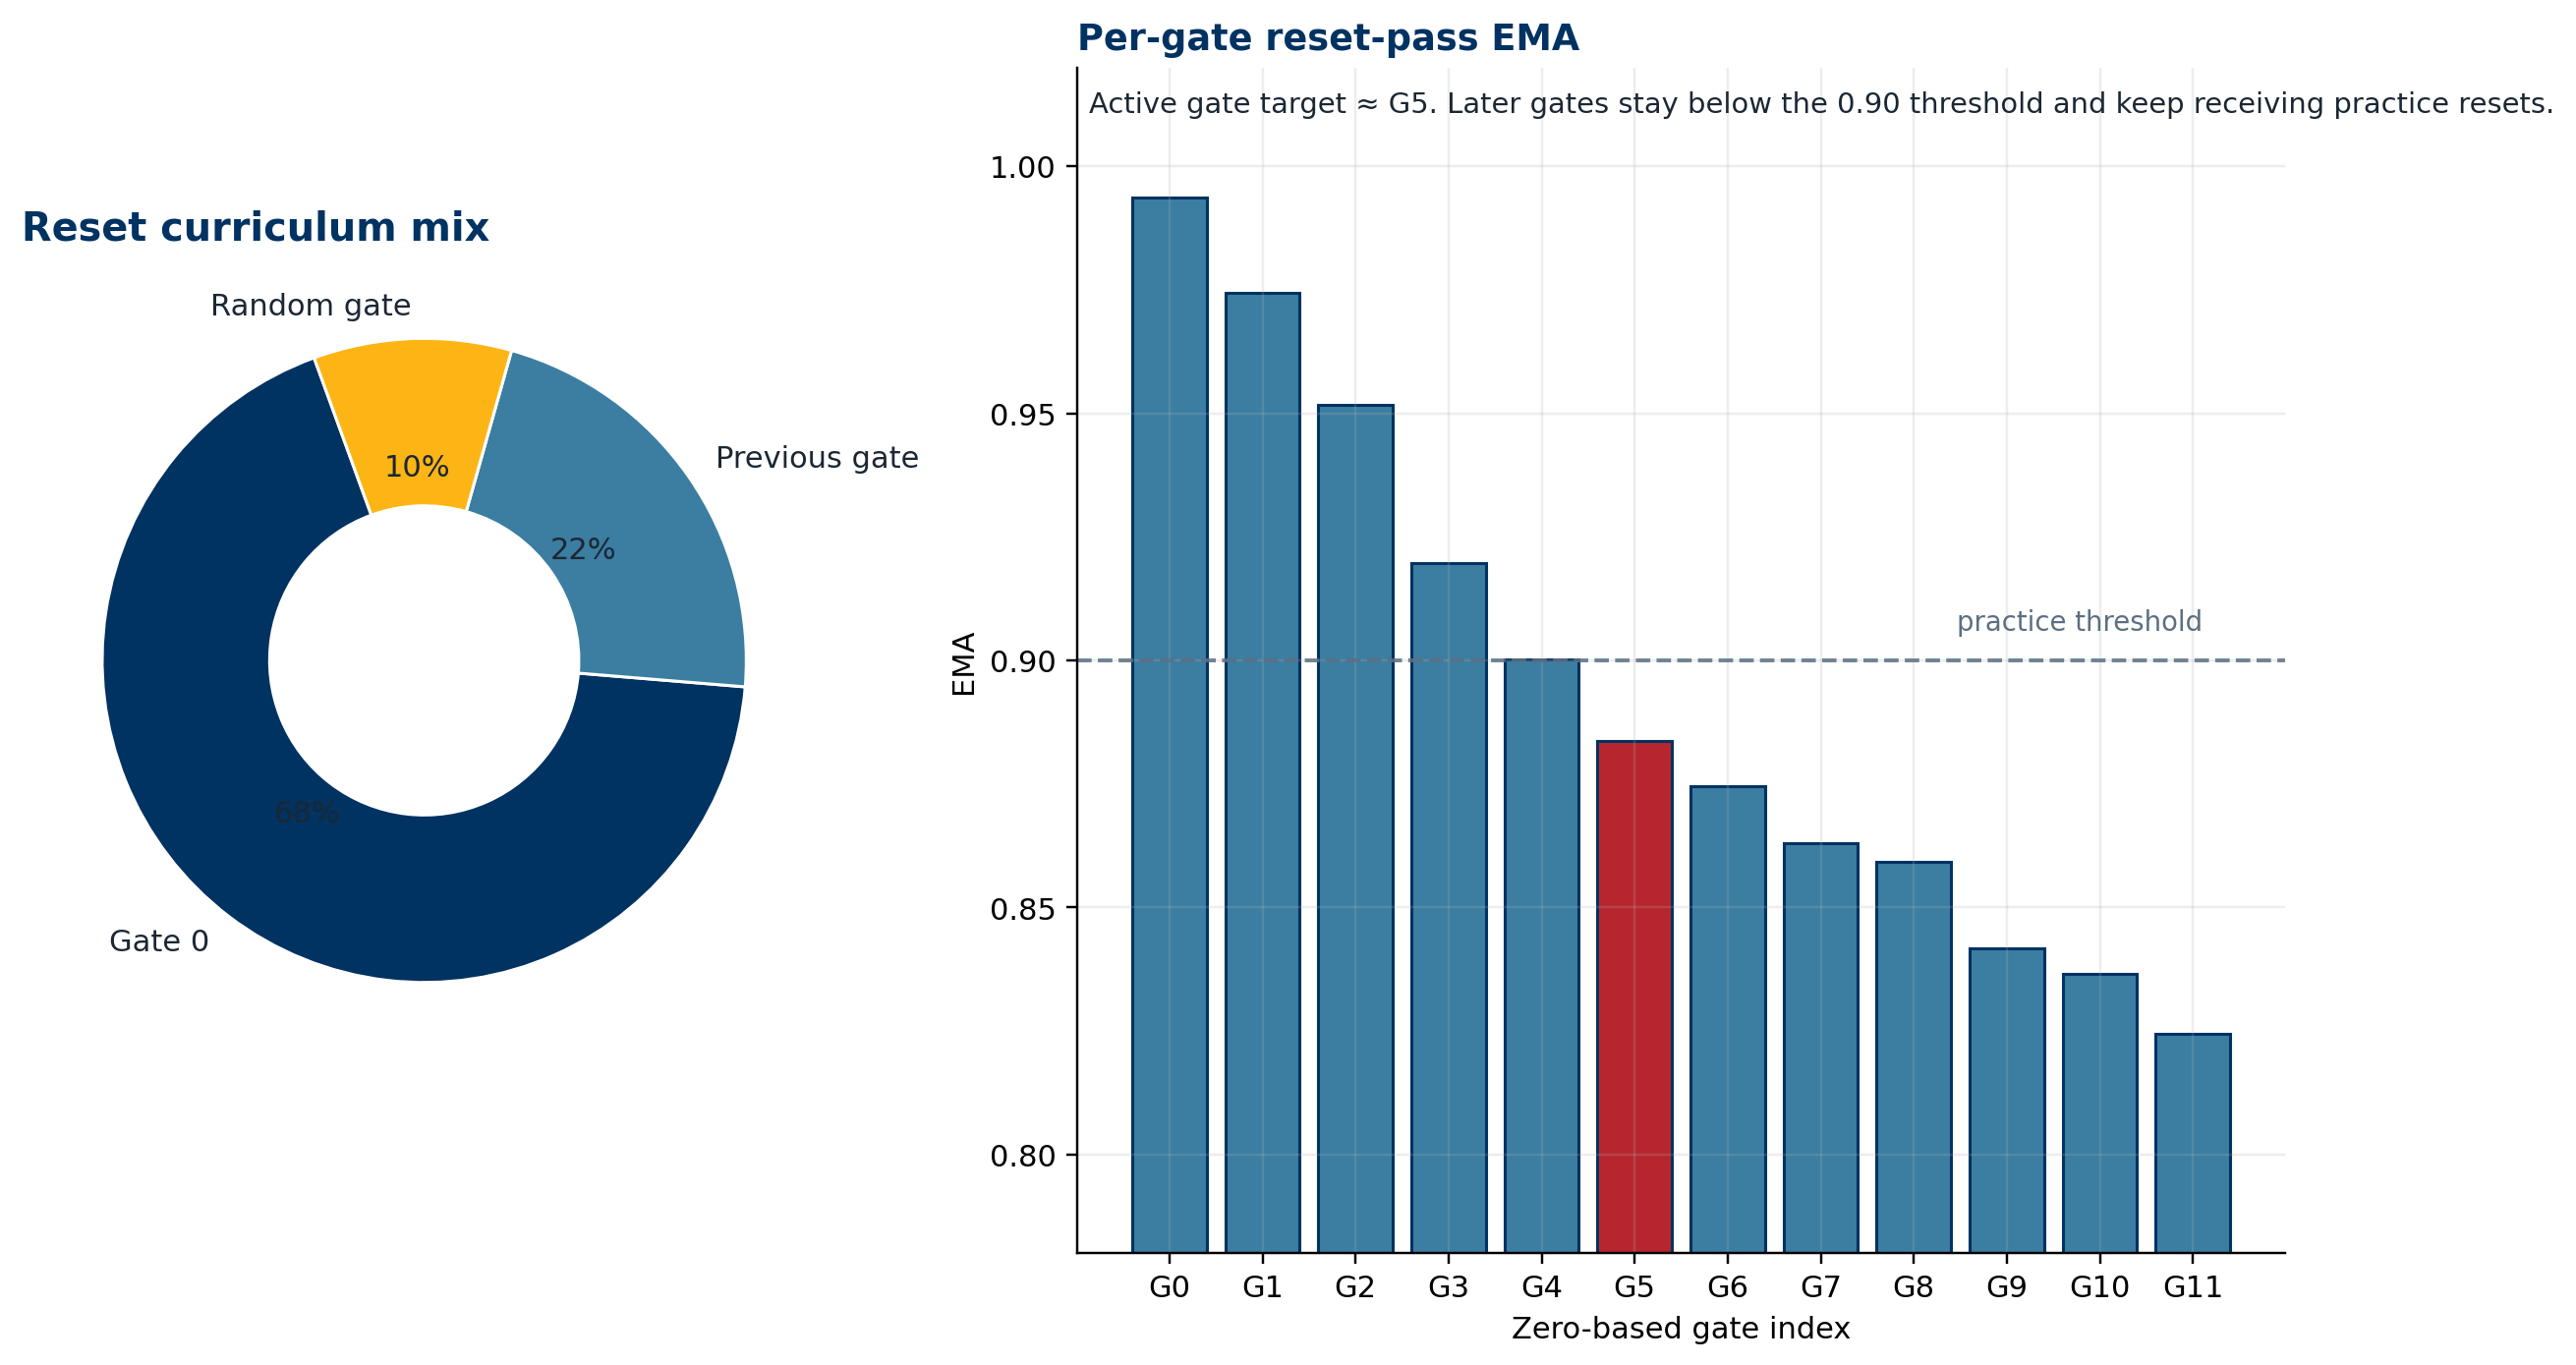
\includegraphics[width=\linewidth]{drone_race_progress_reset_curriculum.png}
    \end{column}
    \begin{column}{0.40\textwidth}
      \begin{block}{Three phases}
        \small
        \begin{itemize}
          \item Phase 0: accuracy-first ordered lap learning.
          \item Phase 1: bridge phase after the first reliable full-lap signal.
          \item Phase 2: speed-focus phase after accuracy crosses the target threshold.
        \end{itemize}
      \end{block}
      \begin{block}{Reset curriculum}
        \small
        The code explicitly allocates resets as 70\% gate 0, 20\% previous gate, and 10\% random gate to keep global course exposure while still drilling the earliest weak bottleneck.
      \end{block}
    \end{column}
  \end{columns}
\end{frame}

\begin{frame}{Network Size and Architecture Evolution}
  \begin{columns}[T,totalwidth=\textwidth]
    \begin{column}{0.60\textwidth}
      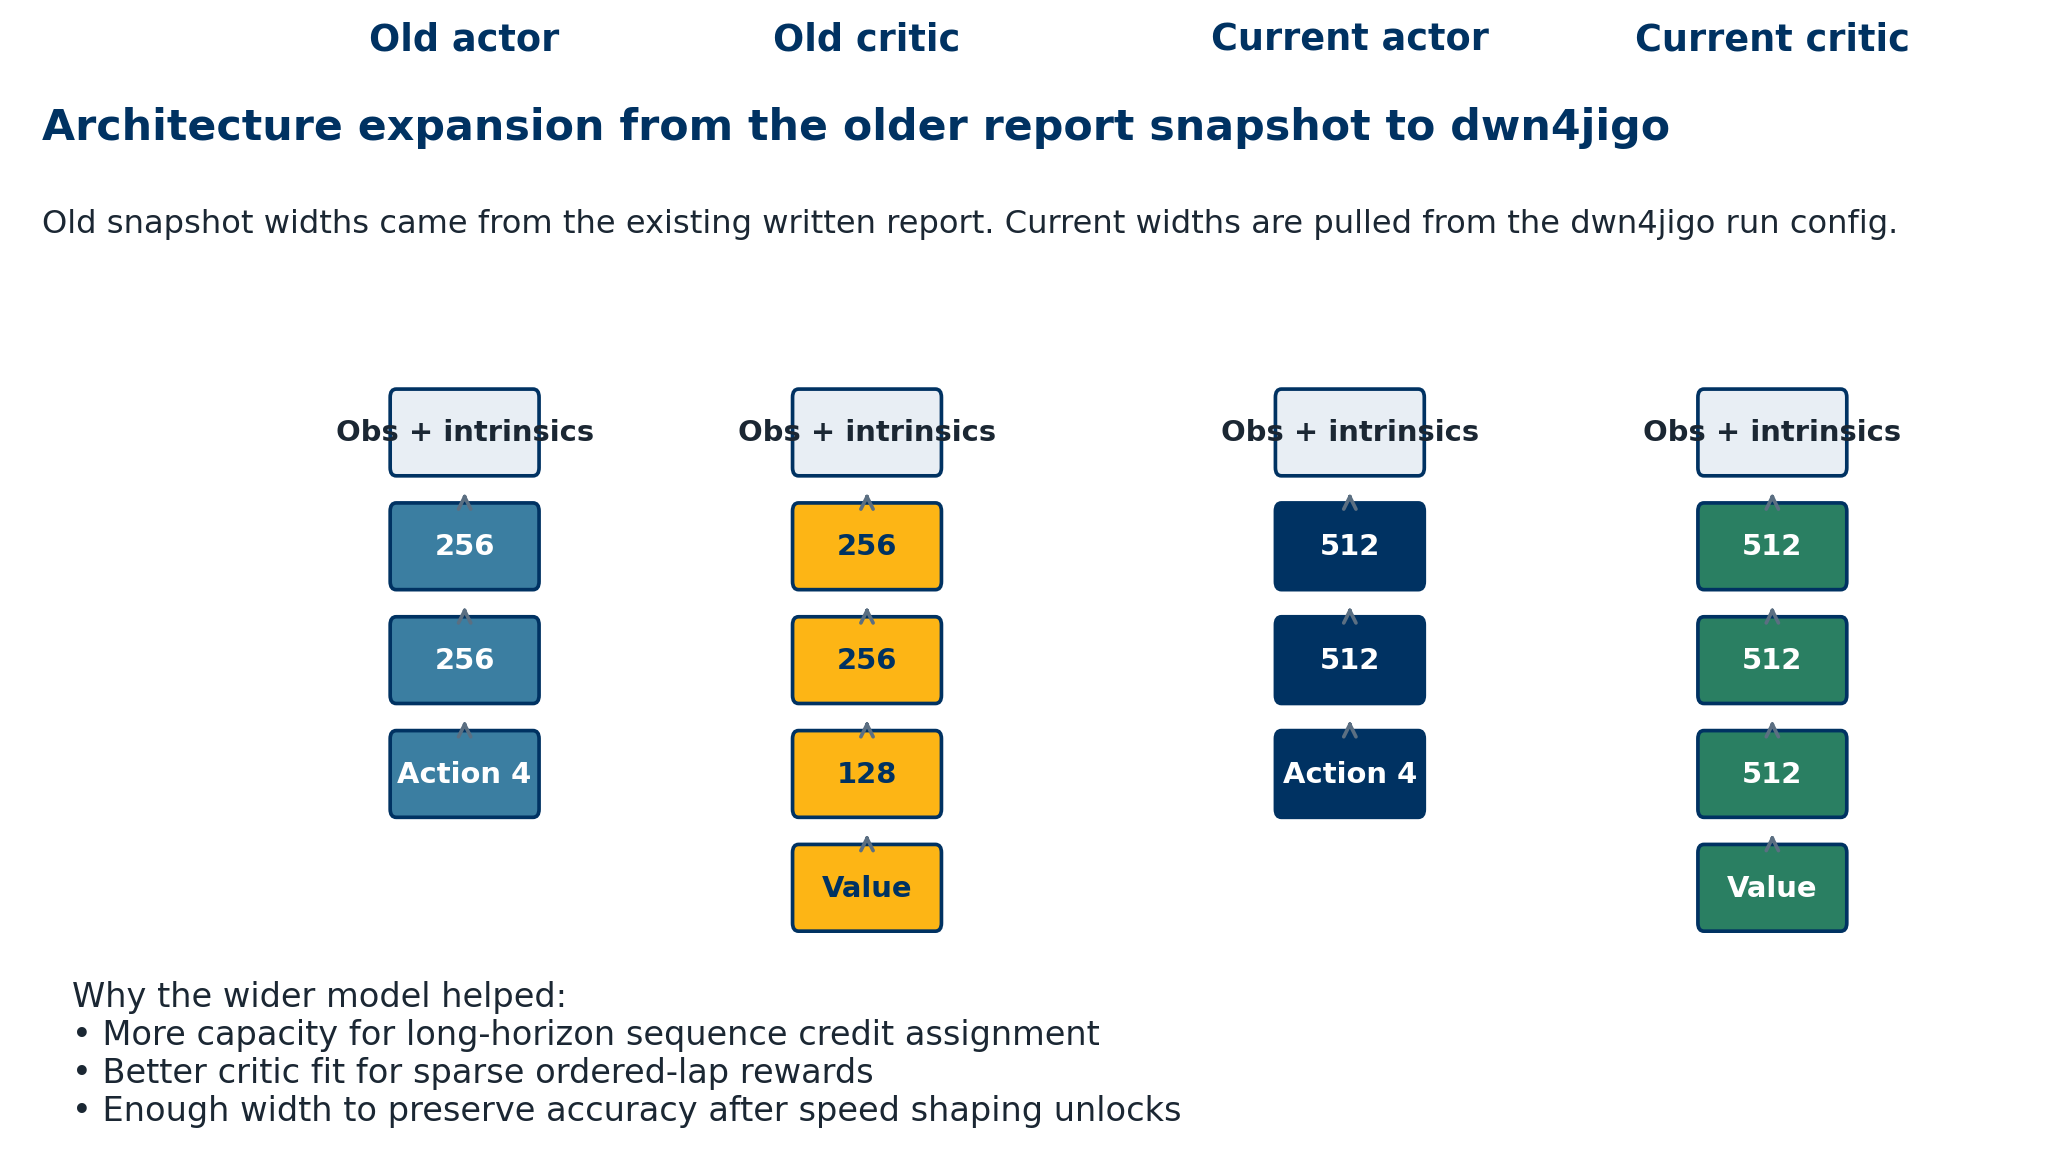
\includegraphics[width=\linewidth]{drone_race_progress_network_architecture.png}
    \end{column}
    \begin{column}{0.38\textwidth}
      \begin{block}{Current widths from \EvidenceRunID}
        \small
        \begin{itemize}
          \item Actor: \texttt{[512, 512]}
          \item Critic: \texttt{[512, 512, 512]}
          \item Activation: LeakyReLU
          \item Layer norm: enabled
        \end{itemize}
      \end{block}
      \begin{block}{Why we widened the model}
        \small
        The critic sees a sparse, sequence-heavy objective. The wider value branch improved fit and reduced the risk that the policy would overreact to noisy early returns.
      \end{block}
    \end{column}
  \end{columns}
\end{frame}

\begin{frame}{Code-Level Novelty That Helped}
  \begin{columns}[T,totalwidth=\textwidth]
    \begin{column}{0.33\textwidth}
      \begin{block}{Gate-center consistency}
        \scriptsize
        \texttt{drone\_race.py}\\[0.2em]
        \texttt{\_get\_gate\_center()} aligns observation, reward, and crossing logic around the aperture center instead of the USD asset origin at the bottom of the gate.
      \end{block}
    \end{column}
    \begin{column}{0.33\textwidth}
      \begin{block}{Stacked reversal handling}
        \scriptsize
        \texttt{stacked\_reversal\_grace\_steps = 220}\\
        \texttt{stacked\_reversal\_dist\_threshold = 35}

        These hooks let the drone survive the local target jump around stacked gates long enough to recover instead of crashing immediately.
      \end{block}
    \end{column}
    \begin{column}{0.33\textwidth}
      \begin{block}{First-class diagnostics}
        \scriptsize
        \texttt{curriculum/reset\_gate\_XX\_pass\_ema}\\
        \texttt{gates/gate\_XX\_crosses}\\
        \texttt{entropy/current\_coef}

        The trainer logs maneuver-level signals, not just return curves, so we can localize failure modes.
      \end{block}
    \end{column}
  \end{columns}
  \vspace{0.5em}
  \begin{beamercolorbox}[wd=\linewidth,sep=0.5ex,rounded=true]{block body}
    \small
    Optional tooling such as auto-stop matters for experiment hygiene, but the main novel pieces that changed learning behavior were the environment-side geometry fixes, reset logic, and richer metrics.
  \end{beamercolorbox}
\end{frame}

\begin{frame}{Results Snapshot from the Evidence Run}
  \small
  \begin{alertblock}{Important reading note}
    This run is the main evidence source for the slide deck, but it predates the final gate-11 accounting fix. We therefore use it for performance trends and for bug interpretation.
  \end{alertblock}
  \vspace{0.4em}
  \begin{columns}[T,totalwidth=\textwidth]
    \begin{column}{0.32\textwidth}
      \metricbox{\LapCompletionPct}{lap completion}
      \vspace{0.5em}
      \metricbox{\GatesPerEpisode}{gates per episode}
    \end{column}
    \begin{column}{0.32\textwidth}
      \metricbox{\LapTimeSeconds}{lap time}
      \vspace{0.5em}
      \metricbox{\MeanSpeedMs}{mean speed}
    \end{column}
    \begin{column}{0.32\textwidth}
      \metricbox{\MaxSpeedMs}{max speed}
      \vspace{0.5em}
      \metricbox{\CrashRatePct}{total crash rate}
    \end{column}
  \end{columns}
\end{frame}

\begin{frame}{Results Trends and Interpretation}
  \begin{columns}[T,totalwidth=\textwidth]
    \begin{column}{0.61\textwidth}
      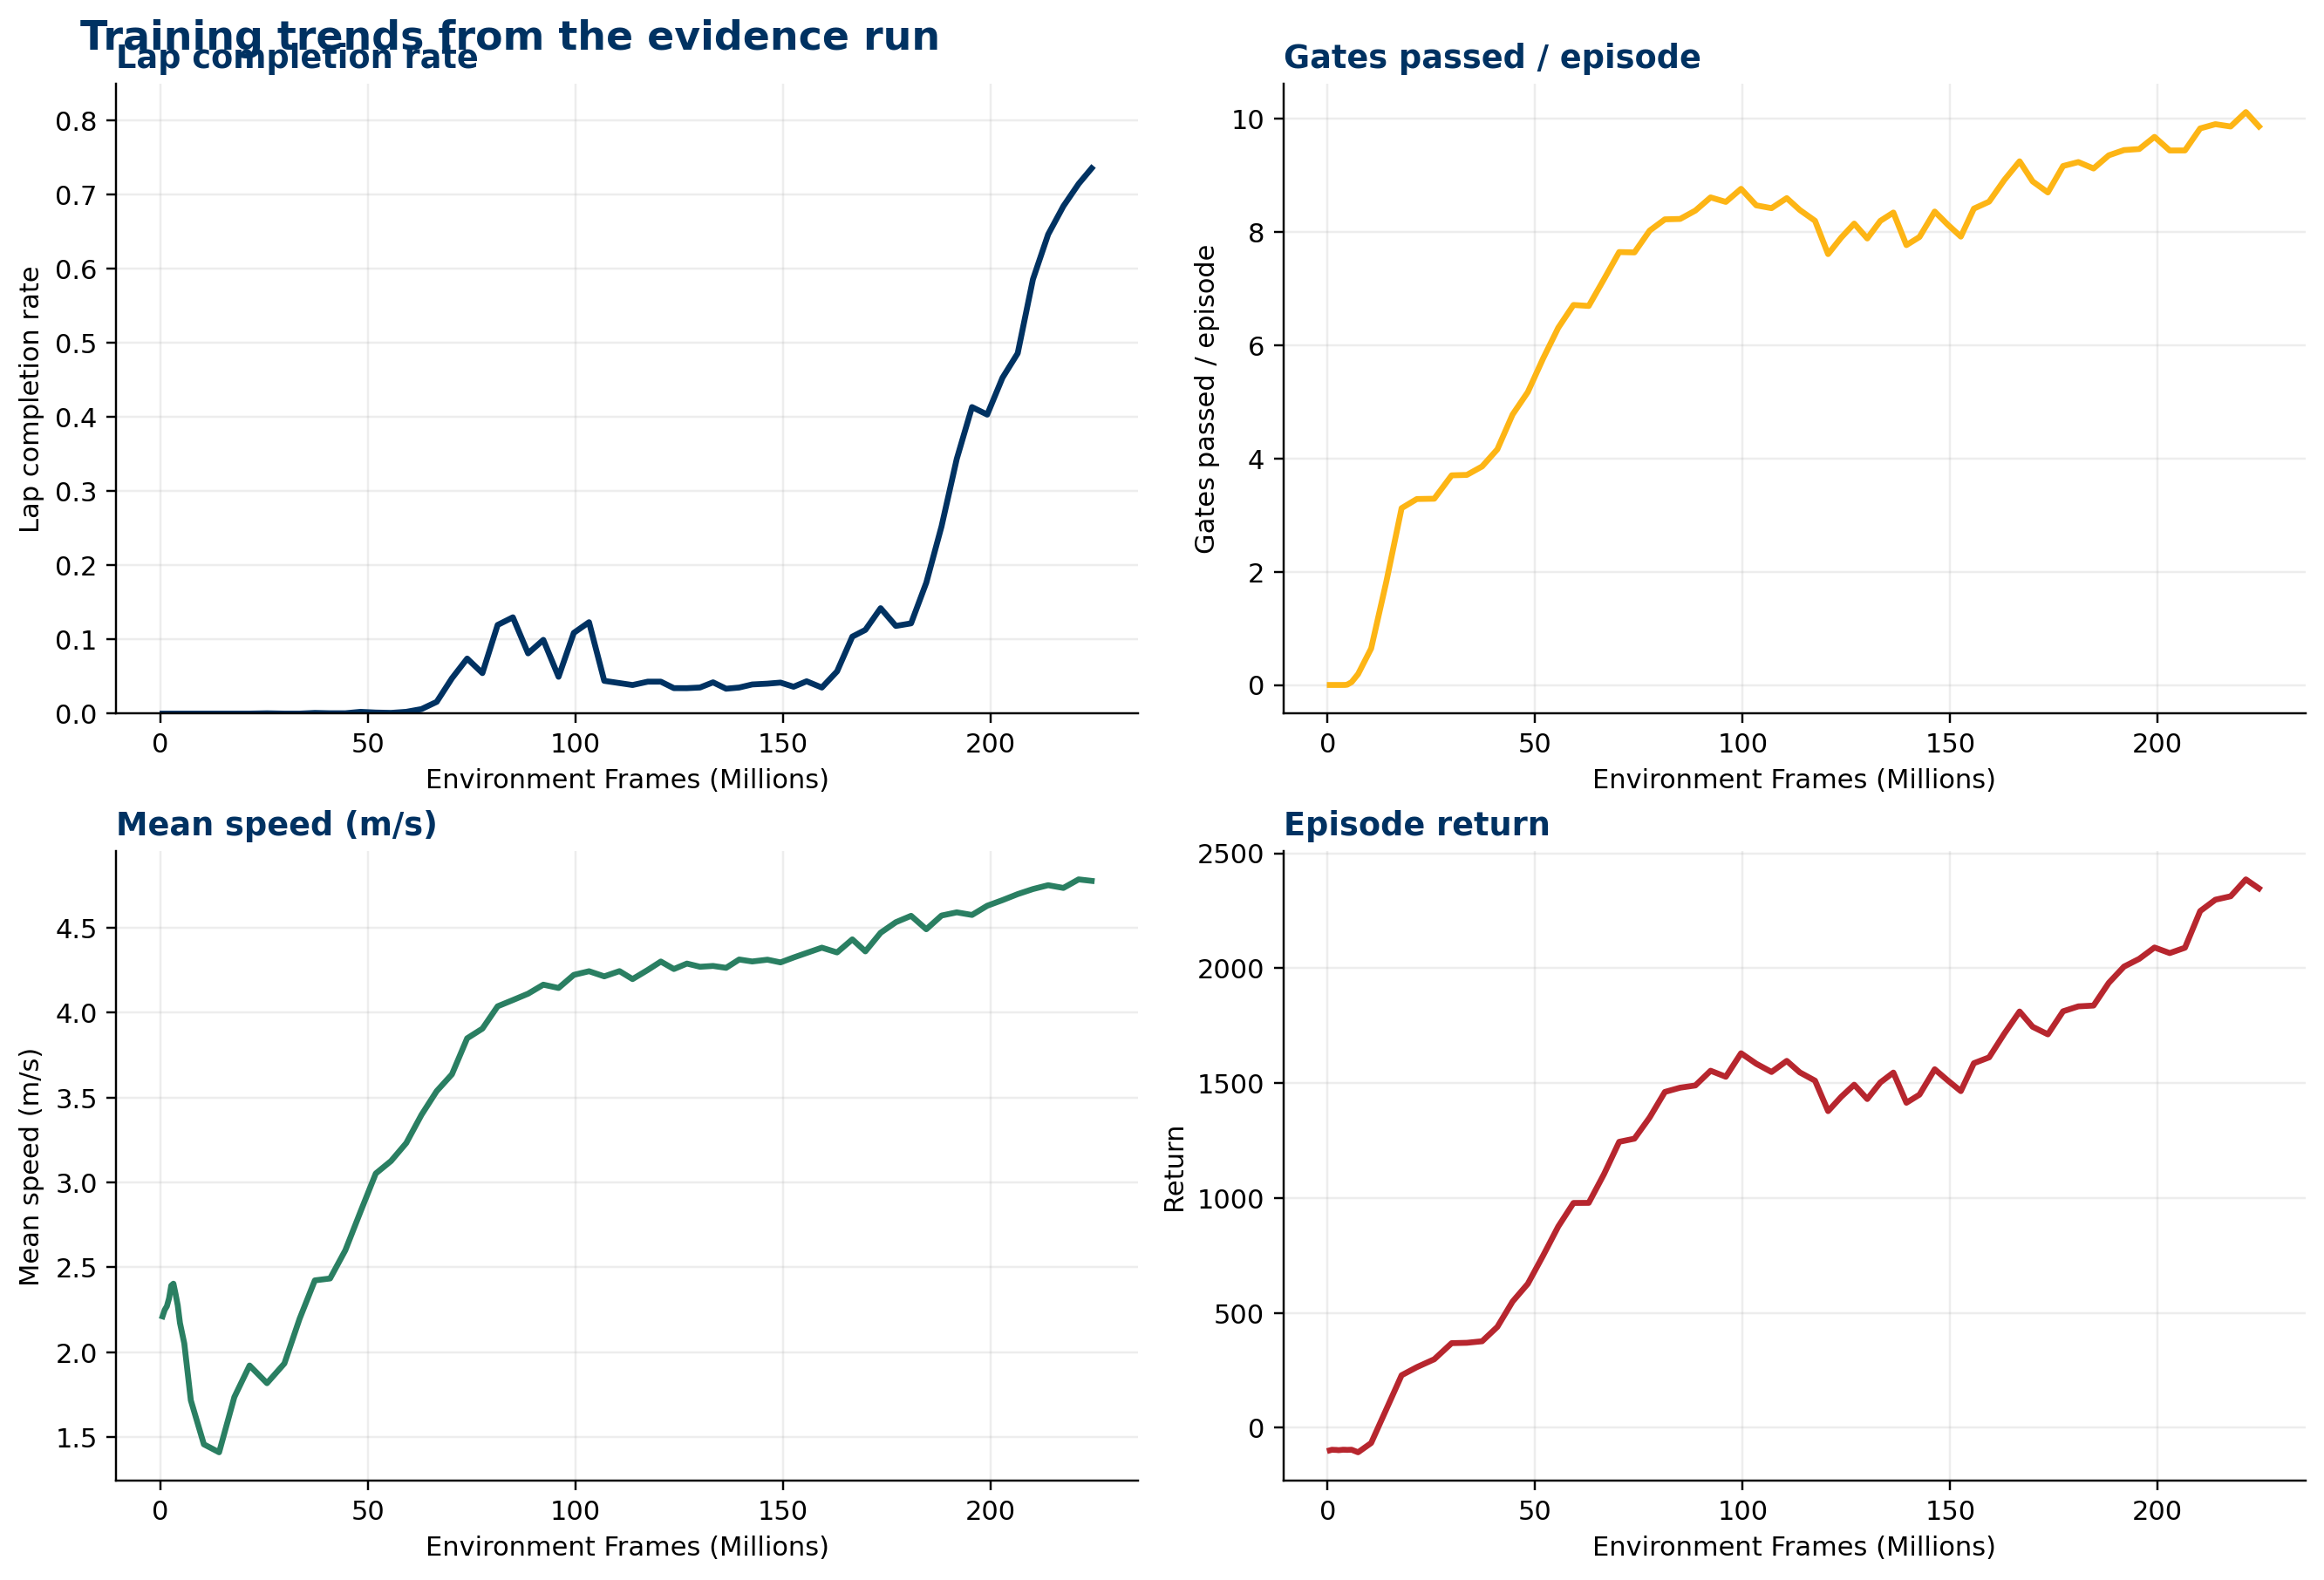
\includegraphics[width=\linewidth]{drone_race_progress_results_trends.png}
    \end{column}
    \begin{column}{0.37\textwidth}
      \begin{block}{What improved together}
        \scriptsize
        \begin{itemize}
          \item Lap completion and gates per episode rise together, so the policy is learning more than a single lucky maneuver.
          \item Mean speed climbs later, after the curriculum shifts toward speed focus.
          \item Return and accuracy stay aligned, which is what we want from an accuracy-first reward hierarchy.
        \end{itemize}
      \end{block}
      \vspace{-0.25em}
      \begin{block}{Interpretation}
        \scriptsize
        By the end of the run, the policy reaches curriculum phase \CurriculumPhase, the accuracy EMA is \AccuracyEMA, and adaptive entropy has decayed to roughly \EntropyCoef. That is the phase-aware exploration decay we were aiming for.
      \end{block}
    \end{column}
  \end{columns}
\end{frame}

\begin{frame}{Per-Gate Analysis and the Gate-11 Bug}
  \begin{columns}[T,totalwidth=\textwidth]
    \begin{column}{0.61\textwidth}
      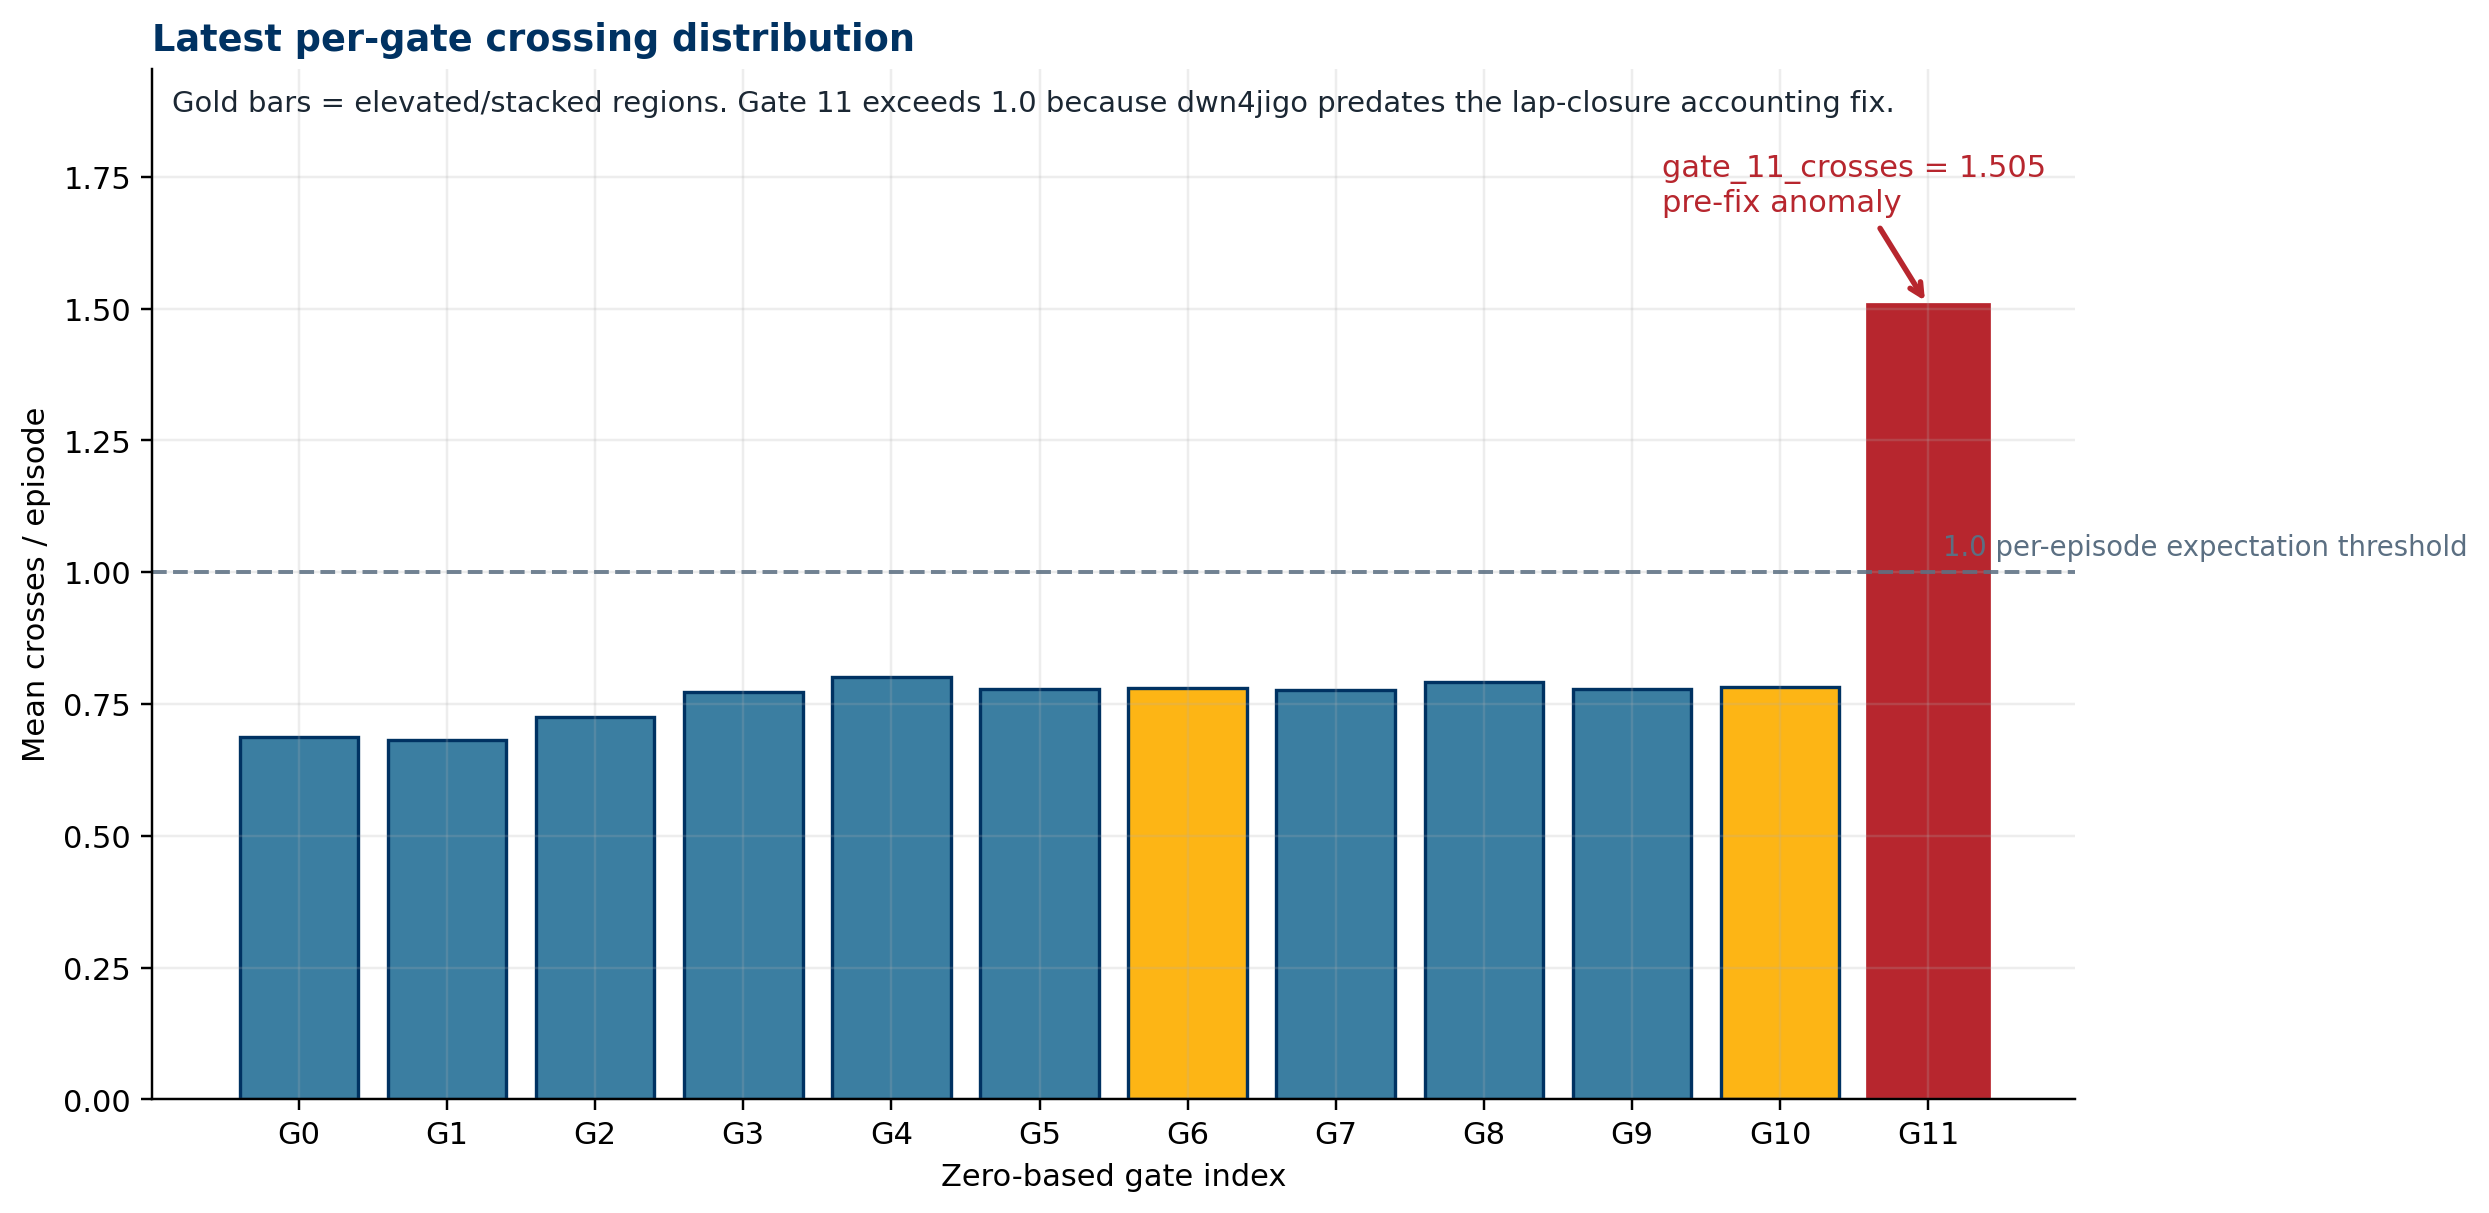
\includegraphics[width=\linewidth]{drone_race_progress_gate_crossings.png}
    \end{column}
    \begin{column}{0.37\textwidth}
      \begin{alertblock}{Anomalous signal}
        \scriptsize
        \texttt{gate\_11\_crosses = \GateElevenCrosses} is not semantically valid as a per-episode gate counter. It should not exceed the expected one-crossing-per-lap bookkeeping.
      \end{alertblock}
      \vspace{-0.25em}
      \begin{block}{Root cause and fix}
        \scriptsize
        The lap-closure implementation used a duplicated final gate entry, and pre-fix accounting allowed the stacked gate-11 region to be counted incorrectly. Commit \texttt{4b808b8} separates the real course gates from the duplicated closure entry so downstream counters ignore the fake lap-closing gate.
      \end{block}
    \end{column}
  \end{columns}
\end{frame}

\begin{frame}{Other Bugs and Lessons Learned}
  \begin{columns}[T,totalwidth=\textwidth]
    \begin{column}{0.49\textwidth}
      \begin{block}{Resolved or partially resolved}
        \small
        \begin{itemize}
          \item \textbf{Gate-center mismatch}: earlier observation and reward logic did not target the exact same physical point as the crossing detector.
          \item \textbf{Immediate post-crossing crashes}: grace windows and stacked-reversal thresholds were necessary so successful crossings did not instantly turn into false divergence terminations.
        \end{itemize}
      \end{block}
      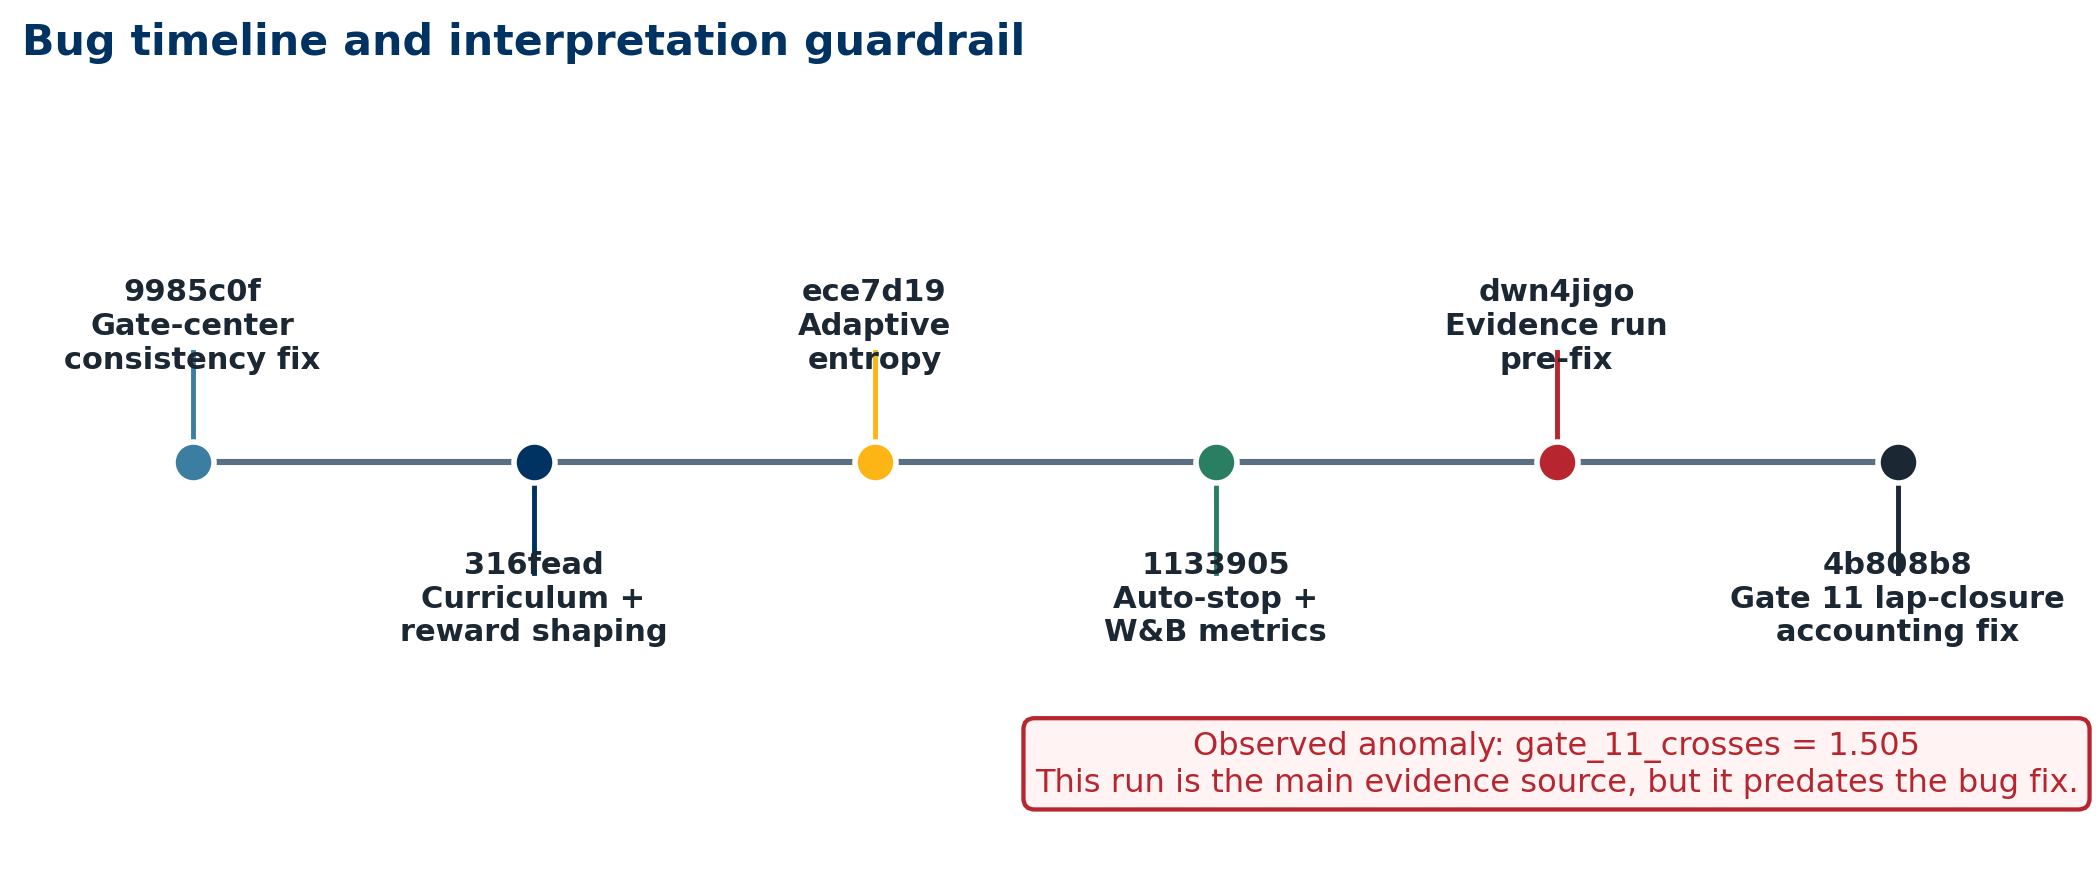
\includegraphics[width=\linewidth]{drone_race_progress_bug_timeline.png}
    \end{column}
    \begin{column}{0.49\textwidth}
      \begin{alertblock}{Still a caveat}
        \scriptsize
        \begin{itemize}
          \item \textbf{Endpoint-only crossing detection}: very fast or awkward local crossings can still be undercounted. A segment-plane intersection test would be more robust.
          \item \textbf{Terminal masking}: PPO GAE currently keys off \texttt{terminated}; once lap completions are common, \texttt{done/truncated} semantics matter more for correct bootstrap behavior.
        \end{itemize}
      \end{alertblock}
      \begin{block}{Main lesson}
        \scriptsize
        Better diagnostics changed how we interpreted training. The biggest wins were not only reward changes, but also enough observability to tell whether the model was missing a maneuver, a metric, or a piece of bookkeeping.
      \end{block}
    \end{column}
  \end{columns}
\end{frame}

\begin{frame}{Planned MPC / TDMPC Direction}
  \begin{columns}[T,totalwidth=\textwidth]
    \begin{column}{0.56\textwidth}
      \begin{block}{What already exists in the repo}
        \small
        \begin{itemize}
          \item \texttt{cfg/algo/tdmpc.yaml} contains a short-horizon TDMPC configuration with CEM planning.
          \item \texttt{omni\_drones/learning/tdmpc.py} already defines the latent dynamics, reward, continuation, and planning code path.
          \item This is a scaffold, not a reported experimental result for DroneRace.
        \end{itemize}
      \end{block}
      \begin{alertblock}{Why we care}
        \small
        A model-based planner is attractive exactly where PPO struggles most: short-horizon stacked reversals, sharp local geometry changes, and situations where one bad target jump can invalidate a purely reactive policy.
      \end{alertblock}
    \end{column}
    \begin{column}{0.42\textwidth}
      \begin{block}{Planned next steps}
        \small
        \begin{itemize}
          \item Re-run after the gate-11 fix and compare the per-gate distribution.
          \item Upgrade gate crossing to a segment-based detector.
          \item Tighten terminal masking around successful lap completion.
          \item Evaluate whether TDMPC can serve as a teacher, warm-start, or direct planner for the stacked reversal bottlenecks.
        \end{itemize}
      \end{block}
      \begin{beamercolorbox}[wd=\linewidth,sep=0.5ex,rounded=true]{block body}
        \small\textbf{Bottom line:} PPO is now strong enough to expose where model-based planning might genuinely help, rather than where reward bugs used to dominate the story.
      \end{beamercolorbox}
    \end{column}
  \end{columns}
\end{frame}

\end{document}
